\graphicspath{{figures/ode/}}

%\setcounter{secnumdepth}{0}
\renewcommand{\theequation}{\thechapter.\arabic{equation}}
\renewcommand{\thetheorem}{\thechapter.\arabic{theorem}}
\renewcommand{\thebc}{\thechapter.\arabic{theorem}}
\renewcommand{\theeg}{\thechapter.\arabic{theorem}}
%\counterwithin{theorem}{chapter}
%\numberwithin{theorem}{chapter}


\chapter{Review of Linear Ordinary Differential Equations}\label{ap:ODE}


\begin{defn}\label{def:apODE}
\begin{enumerate}[(a)]
\item %%% (a)
A \emph{differential equation} is an equation for an
unknown function that contains the derivatives of that unknown function.
For example $y''(t)+y(t)=0$ is a differential equation for the unknown 
function $y(t)$.

\item %% (b) 
A differential equation is called an \emph{ordinary differential
equation} (often shortened to ``ODE'') if only ordinary derivatives 
appear. That is, if the unknown function has only a single independent
variable. A differential equation is called a \emph{partial differential
equation} (often shortened to ``PDE'') if partial derivatives 
appear. That is, if the unknown function has more than one independent
variable. For example $y''(t)+y(t)=0$ is an ODE while
$\frac{\partial^2 u}{\partial\, t^2}(x,t)=c^2 
\frac{\partial^2 u}{\partial\, x^2}(x,t)$ is a PDE.

\item %% (c) 
The \emph{order} of a differential equation is the order of the
highest derivative that appears. For example $y''(t)+y(t)=0$ 
is a second order ODE.

\item %% (d) 
An ordinary differential equation that is of the form
\begin{equation}\label{eqn:ODEordern}
a_0(t) y^{(n)}(t) + a_1(t) y^{(n-1)}(t)+\cdots+a_{n-1}(t) y'(t) +a_n(t)y(t)
=F(t)
\end{equation}
with given coefficient functions $a_0(t)$, $\cdots$, $a_n(t)$ and $F(t)$ 
is said to be \emph{linear}. Otherwise, the ODE is said to be \emph{nonlinear}.
For example, $y'(t)^2+y(t)=0$, $y'(t)y''(t)+y(t)=0$ and $y'(t)=e^{y(t)}$
are all nonlinear.

\item %% (e) 
The ODE \eqref{eqn:ODEordern} is said to have \emph{constant coefficients} if
the coefficients  $a_0(t)$, $a_1(t)$, $\cdots$, $a_n(t)$ are all constants. Otherwise,
it is said to have \emph{variable coefficients}. For example,
the ODE $y''(t)+7y(t)=\sin t$ is constant coefficient, while 
$y''(t)+ty(t)=\sin t$ is variable coefficient.

\end{enumerate}
\end{defn}

\addtocounter{theorem}{-1}
\begin{defn}[continued]
\begin{enumerate}[(a)]

\item[(f)] %% (f) 
The ODE \eqref{eqn:ODEordern} is said to be \emph{homogeneous} if $F(t)$ 
is identically zero. Otherwise, it is said to be \emph{inhomogeneous} or 
\emph{nonhomogeneous}. For example, the ODE $y''(t)+7y(t)=0$ is homogeneous, 
while  $y''(t)+7y(t)=\sin t$ is inhomogeneous. A homogeneous ODE always
has the trivial solution $y(t)=0$.

\item[(g)] %% (g) 
An \emph{initial value problem}  is a problem in which one is to find
an unknown function $y(t)$ that satisfies both a given ODE and given
initial conditions, like $y(t_0)=1$, $y'(t_0)=0$. Note that all of the 
conditions involve the function $y(t)$ (or its derivatives) evaluated at 
a single time $t=t_0$.

\item[(h)] %% (h) 
A \emph{boundary value problem}  is a problem in which one is to find
an unknown function $y(t)$ that satisfies both a given ODE and given
boundary conditions, like $y(t_0)=0$, $y(t_1)=0$. Note that the conditions 
involve the function $y(t)$ (or its derivatives) evaluated at two different 
times. 


\end{enumerate}
\end{defn}


\noindent The following theorem gives the form of solutions to the ODE
\eqref{eqn:ODEordern}.

\begin{theorem}\label{thm:odeMain}
Assume that the coefficients $a_0(t)$, $a_1(t)$, $\cdots$, $a_{n-1}(t)$, 
$a_n(t)$ and $F(t)$ are continuous functions and that 
$a_0(t)$ is not zero.

\begin{enumerate}[(a)]
\item %% (a) 
The general solution to the ODE \eqref{eqn:ODEordern} is of the form
\begin{equation}\label{eqn:ODEgensln}
y(t)=y_p(t)+ C_1y_1(t)+C_2y_2(t)+\cdots+C_n y_n(t)
\end{equation}
where 
\begin{itemize}\itemsep1pt \parskip0pt \parsep0pt %\itemindent-15pt
\item[$\circ$] $n$ is the order of \eqref{eqn:ODEordern}
\item[$\circ$] $y_p(t)$ is any solution to \eqref{eqn:ODEordern}
\item[$\circ$] $C_1$, $C_2$, $\cdots$, $C_n$ are arbitrary constants
\item[$\circ$] $y_1$, $y_2$, $\cdots$, $y_n$ are $n$ independent solutions
to the homogenous equation 
\begin{equation*}
a_0(t) y^{(n)}(t) + a_1(t) y^{(n-1)}(t)+\cdots+a_{n-1}(t) y'(t) +a_n(t)y(t)=0
\end{equation*}
associated to \eqref{eqn:ODEordern}.
``Independent'' just means that no $y_i$ can be written as a linear combination
of the other $y_j$'s. For example, $y_1(t)$ cannot be expressed in the form
$b_2y_2(t)+\cdots+b_ny_n(t)$. 
\end{itemize}
In \eqref{eqn:ODEgensln}, $y_p$ is called the ``particular solution'' and 
$C_1y_1(t)+C_2y_2(t)+\cdots+C_n y_n(t)$ is called the 
``complementary solution''.

\end{enumerate}
\end{theorem}

\addtocounter{theorem}{-1}
\begin{theorem}[continued]
\begin{enumerate}[(a)]

\item[(b)] %% (b) 
Given any constants $b_0$, $\cdots$, $b_{n-1}$ there is exactly
one function $y(t)$ that obeys the ODE \eqref{eqn:ODEordern} and the initial
conditions
\begin{equation*}
y(0)=b_0\qquad y'(0)=b_1\qquad \cdots\qquad y^{(n-1)}(0)=b_{n-1}
\end{equation*}
\end{enumerate}
\end{theorem}

\begin{eg}[RLC circuit]\label{eg:RLC}
As an example of the most commonly used techniques for solving linear,
constant coefficient ODE's, we consider the RLC circuit, which is
the electrical circuit consisting of a resistor of
resistance $R$, a coil (or solenoid) of inductance $L$, a capacitor 
of capacitance $C$ and a voltage source arranged in series, as shown below. 
Here $R$, $L$
and $C$ are all nonnegative constants.
\begin{efig}
\begin{center}
    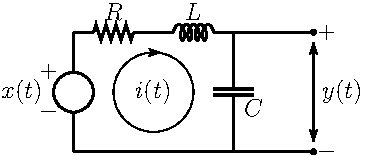
\includegraphics[scale=1.3]{RLC.pdf}
\end{center}
\end{efig}
 We're going to think of the voltage $x(t)$ as an input signal,
and the voltage $y(t)$ as an output signal. 
The goal is to determine the output signal produced by a given input signal. 
If $i(t)$ is the current flowing at time $t$ in the loop as shown and 
$q(t)$ is the charge on the capacitor, then the voltages across $R$, $L$ 
and $C$, respectively, at time $t$ are
$Ri(t)$, $L\diff{i}{t}(t)$ and $y(t)=\frac{q(t)}{C}$. By the Kirchhoff's 
law\footnote{Gustav Robert Kirchhoff (1824--1887) was a German physicist.} 
that says that the voltage between any two points has to be independent 
of the path used to travel between the two points, these three voltages 
must add up to $x(t)$ so that
\begin{equation}\label{eqn:RLCrlc}
Ri(t) + L\diff{i}{t}(t) + \frac{q(t)}{C} = x(t)
\end{equation}
Assuming that $R,\ L,\ C$ and $x(t)$ are known, this is still one 
differential equation in two unknowns, $i(t)$ and $q(t)$. Fortunately,
there is a relationship between the two. Namely
\begin{equation}\label{eqn:RLCiq}
i(t)=\diff{q}{t}(t) = Cy'(t)
\end{equation}
This just says that the capacitor cannot create or destroy charge on 
its own; all charging of the capacitor must come from the current.  
Substituting \eqref{eqn:RLCiq} into \eqref{eqn:RLCrlc} gives
\begin{equation*}%\label{eqn:RLCxyode}
 LCy''(t) + RCy'(t) + y(t) = x(t)
\end{equation*}
As a concrete example, we'll take  an ac voltage source and choose the 
origin of time so that $x(0)=0$, $x(t)=E_0\sin(\om t)$. Then the differential equation becomes
\refstepcounter{equation}\label{eqn:ODERy}
\begin{equation}\tag{\ref{eqn:ODERy}}
LCy''(t)+RCy'(t)+y(t)=E_0\sin(\om t)
\end{equation}
This is a second order, linear, constant coefficient ODE. So we know, 
from Theorem \ref{thm:odeMain}, that the general solution is of the form 
$y_p(t)+C_1y_1(t)+C_2y_2(t)$, where 
\begin{itemize}\itemsep1pt \parskip0pt \parsep0pt %\itemindent-15pt
\item[$\circ$]
 $y_p(t)$, the particular solution, is any one solution
to  \eqref{eqn:ODERy},
\item[$\circ$]
$C_1,C_2$ are arbitrary
constants and 
\item[$\circ$]
$y_1(t)$, $y_2(t)$ are any two independent solutions of the corresponding
homogeneous equation
\begin{equation}\tag{\ref{eqn:ODERy}$_{\rm h}$}
LCy''(t)+RCy'(t)+y(t)=0
\end{equation}
\end{itemize}
So to find the general solution to \eqref{eqn:ODERy}, we need to find 
three functions: $y_1(t)$, $y_2(t)$ and $y_p(t)$.

\medskip
%%%%%%%%%%%%%%%%%%%%%%%%
\begin{itemize}
\item
\emph{Finding $y_1(t)$ and $y_2(t)$:}\ \ \ 
The best way to find $y_1$ and $y_2$ is to guess them. 
Any solution, $y_h(t)$, of 
(\ref{eqn:ODERy}$_{\rm h}$) has to have the property that $y_h(t)$, $RCy_h'(t)$ and 
$LCy_h''(t)$ cancel each other out for all $t$. We choose our guess 
so that $y_h(t)$, $y_h'(t)$ and $y_h''(t)$ are all proportional to a single 
function of $t$. Then it will be easy to see if $y_h(t)$, $RCy_h'(t)$ and 
$LCy_h''(t)$ all cancel. All derivatives of the function $e^{rt}$ are again proportional to $e^{rt}$. Hence we try $y_h(t)=e^{rt}$, with the constant
$r$ to the determined. This guess is a solution of (\ref{eqn:ODERy}$_{\rm h}$) 
if and only if
\begin{equation}\label{eqn:ODERroots}
\begin{split}
LCr^2e^{rt}+RCre^{rt}+e^{rt}=0
&\iff LCr^2+RCr+1 =0 \\
&\iff  r=\frac{-RC\pm\sqrt{R^2C^2-4LC}}{2LC}\equiv r_{1,2}
\end{split}
\end{equation}
How we proceed depends on the sign of $R^2C^2-4LC$. That is, whether
$R> 2\sqrt{\frac{L}{C}}$ or  $R< 2\sqrt{\frac{L}{C}}$
or $R = 2\sqrt{\frac{L}{C}}$.
%%%%%%%%%%%
\begin{itemize}
\item 
\emph{Finding $y_1(t)$ and $y_2(t)$, when $R> 2\sqrt{\frac{L}{C}}$:}\ \ \ 
Then $R^2C^2-4LC> 0$, and $r_1$ and $r_2$ are two different real numbers. 
We may take $y_1(t)=e^{r_1t}$ and $y_2(t)=e^{r_2t}$ so that 
the complimentary solution is 
$
C_1y_1(t)+C_2y_2(t)=C_1 e^{r_1t}+C_2e^{r_2 t}
$. 
\smallskip%%%%%
\item 
\emph{Finding $y_1(t)$ and $y_2(t)$, when $R< 2\sqrt{\frac{L}{C}}$:}\ \ \ 
Then $R^2C^2-4LC< 0$ and $r_1$ and $r_2$
are the two different complex numbers $-\rho\pm i\nu$, where 
\begin{equation*}
\rho=\frac{R}{2L}\qquad\text{and}\qquad
 \nu=\frac{\sqrt{4LC-R^2C^2}}{2LC}
\end{equation*} 
We may again take 
$
C_1 e^{r_1t}+C_2e^{r_2 t}
$
as the complimentray solution.  However we can also rewrite
$C_1 e^{r_1t}+C_2e^{r_2 t}$ in terms of real valued functions 
by using that $e^{\pm i\theta}=\cos\theta\pm i\sin\theta$:
\begin{align*}
C_1 e^{r_1t}+C_2e^{r_2 t} 
  &=e^{-\rho t}\big[C_1e^{i\nu t}+C_2e^{-i\nu t}\big]\\
  &=e^{-\rho t}\big[C_1\big\{\cos(\nu t)+i\sin(\nu t)\big\}+
               C_2\big\{\cos(\nu t)-i\sin(\nu t)\big\}\big]\\
  &=e^{-\rho t}\big[D_1\cos(\nu t)+D_2\sin(\nu t)\big]
\end{align*}
where\footnote{Don't make the mistake of thinking that $C_1$ 
and $C_2$ have to be real numbers, forcing $D_2$ to be pure  imaginary. 
In most applications, $D_1$ and $D_2$ will be pure real and $C_1$ and 
$C_2$ will be complex.} $D_1=C_1+C_2,\ D_2=i(C_1-C_2)$. So we may also take 
$y_1(t)=e^{-\rho t}\cos(\nu t)$, $y_2(t)=e^{-\rho t}\sin(\nu t)$ in 
the complementary solution. 

There is yet a third useful way to write 
the complementary solution.
Think of $(D_1,D_2)$ as a point in the $xy$-plane. Call the polar
coordinates of that point $A$ and $\theta$ so that $D_1=A\cos\theta$ and 
$D_2=A\sin\theta$. Then, using the trig identity $\cos(\alpha+\beta)
=\cos \alpha\cos\beta-\sin \alpha\sin \beta$, with $\alpha=\nu t$ and $\beta=-\theta$,
\begin{equation}\label{eqn:RLCampPhase}
\begin{split}
e^{-\rho t}\big[D_1\cos(\nu t)+D_2\sin(\nu t)\big]
&=e^{-\rho t}\big[A\cos(\nu t)\cos\theta+A\sin(\nu t)\sin\theta\big]\\
&=Ae^{-\rho t}\cos(\nu t-\theta)
\end{split}
\end{equation}
We have, in effect, replaced the two arbitrary constants $D_1$ and $D_2$,
whose values would normally be determined by initial conditions, by two
other arbitrary constants, $R$ and $\theta$, whose values would also normally 
be determined by initial conditions. 
\smallskip%%%%%
\item 
\emph{Finding $y_1(t)$ and $y_2(t)$, when $R=2\sqrt{\frac{L}{C}}$:}\ \ \ 
Then $R^2C^2-4LC=0$ so that $r_1=r_2$. We may take
$y_1=e^{r_1t}$, but $e^{r_2t}=e^{r_1t}$ is certainly not a second independent
solution. So we still need to find $y_2$.  
Here is a trick (called reduction of order\footnote{The modern method of reduction of order was created by the French mathematician, physicist 
and music theorist Jean le Rond d'Alembert (1717-1783). The interested reader
can easily search out more about his life.}) for finding 
the other solutions:
look for solutions of the form  $v(t)e^{-r_1 t}$. Here $e^{-r_1 t}$
is the solution we have already found and $v(t)$ is to be determined.
To save writing, set $\rho=\frac{R}{2L}$ so that $r_1=r_2=\rho$.
To save writing also divide (\ref{eqn:ODERy}$_{\rm h}$) by $LC$ and 
substitute that $\frac{R}{L}=2\rho$ and  
$\frac{1}{LC}=\frac{R^2}{4L^2}=\rho^2$.  (Recall that we are assuming 
that $R^2=\frac{4L}{C}$.) So (\ref{eqn:ODERy}$_{\rm h}$) is equivalent to
\begin{equation*}
y_h''(t)+2\rho\,y_h'(t)+\rho^2\,y_h(t)=0
\end{equation*}
Substitute in 
\begin{align*}
y_h(t)&=\ \ \  v(t)e^{-\rho t}\\
y_h'(t)&= -\rho v(t)e^{-\rho t}+\phantom{2\rho}v'(t)e^{-\rho t}\\
y_h''(t)&= \phantom{-}\rho^2 v(t)e^{-\rho t}-2\rho v'(t)e^{-\rho t}
                  +v''(t)e^{-\rho t}
\end{align*}
So when $y_h(t)=v(t)e^{-\rho t}$,
\begin{align*}
&y_h''(t)+2\rho\,y_h'(t)+\rho^2\,y_h(t)\\
&\hskip1in=\big[\rho^2\!-\!2\rho^2\!+\!\rho^2\big]v(t)e^{-\rho t}
       +\big[-2\rho\!+\!2\rho\big]v'(t)e^{-\rho t}+v''(t)e^{-\rho t}\\
&\hskip1in=v''(t)e^{-\rho t}
\end{align*}
Thus $v(t)e^{-\rho t}$ is a solution of (\ref{eqn:ODERy}$_{\rm h}$) whenever the function
$v''(t)=0$ for all $t$. But, for any values of the constants $C_1$ and $C_2$, 
$v(t)=C_1+C_2t$ has vanishing second derivative
so $\big(C_1+C_2t\big)e^{-\rho t}=\big(C_1+C_2t\big)e^{-r_1 t}$ solves 
(\ref{eqn:ODERy}$_{\rm h}$). This is of the form  $C_1y_1(t)+C_2y_2(t)$ with
$y_1(t)=e^{-r_1t}$, the solution that we found first, and $y_2(t)=te^{-r_1t}$,
a second independent solution. So we may take $y_2(t)=te^{r_1t}$.

\end{itemize}
%%%%%%%%%%%%%%%%%%%%%%%%%%%%%%%%%%%%%%%%%%
\item
\emph{Finding $y_p(t)$:}\ \ \ 
The best way to find $y_p$ is to guess it. We guess that the circuit 
responds to an oscillating input voltage with an output voltage that oscillates 
at the same frequency. So we try 
$y_p(t)=\mathcal{A}\sin(\om t-\varphi)$ with the amplitude $\mathcal{A}$ 
and phase $\varphi$ to be determined. 

For $y_p(t)$ to be a solution, we need
\begin{align*}
LCy_p''(t)+RCy_p'(t)+y_p(t)
   &=E_0 \sin(\om t)\\
-LC\om^2\mathcal{A}\sin(\om t-\varphi)+RC\om \mathcal{A}\cos(\om t-\varphi)
+\mathcal{A}\sin(\om t-\varphi)
&=E_0 \sin(\om t)\\
&=E_0 \sin(\om t-\varphi+\varphi)
\end{align*}
and hence, applying $\sin(A+B)=\sin A\cos B+\cos A\sin B$ with $A=\om
t-\varphi$ and $B=\varphi$,
\begin{align*}
&\big(1-LC\om^2\big)\mathcal{A}\sin(\om t-\varphi)+RC\om \mathcal{A}\cos(\om t-\varphi)
\\&\hskip2in
=E_0 \cos(\varphi)\sin(\om t-\varphi)
+ E_0 \sin(\varphi)\cos(\om t-\varphi)
\end{align*}
Matching coefficients of $\sin(\om t-\varphi)$ and $\cos(\om t-\varphi)$ on 
the left and right hand sides gives
\begin{align}
\big(1-LC\om^2\big)\mathcal{A}&= E_0 \cos(\varphi)\label{eqnODERnum}\\
RC\om \mathcal{A}&=E_0 \sin(\varphi)\label{eqnODERden}
\end{align}
It is now easy to solve for $\mathcal{A}$ and $\varphi$
\begin{alignat*}{3}
\frac{\eqref{eqnODERden}}{\eqref{eqnODERnum}}
&\implies \tan(\varphi) = \frac{RC\om}{1-LC\om^2}\\
&\implies \varphi = \arctan\frac{RC\om}{1-LC\om^2}\\[0.1in]
\sqrt{\eqref{eqnODERnum}^2\!+\eqref{eqnODERden}^2}
&\implies\sqrt{\big(1\!-\!LC\om^2\big)^2+R^2C^2\om^2}\ \mathcal{A}= E_0 \\
&\implies \mathcal{A}=\frac{E_0}{\sqrt{(1\!-\!LC\om^2)^2+R^2C^2\om^2}}
\end{alignat*}
\end{itemize}
Naturally, different input frequencies $\om$ give different output 
amplitudes $\mathcal{A}$. Here is a graph of $\mathcal{A}$ against $\om$, 
with all other parameters held fixed.
\begin{nfig}
\begin{center}
    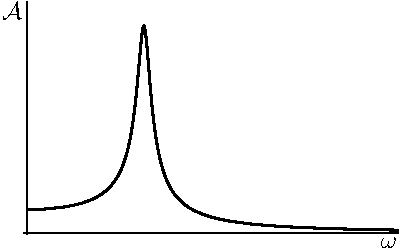
\includegraphics{resonance.pdf}
\end{center}
\end{nfig}
Note that there is a small range of frequencies that give a large
amplitude response. This is the phenomenon of resonance. It is exploited
in the design of radio and television tuning circuitry. It has also been
dramatically illustrated in, for example, the collapse\footnote{There are videos of the collapse on the web.} of the Tacoma narrows bridge. 
\end{eg}

\begin{eg}[Boundary Value Problems]\label{exBVP}
By part (b) of Theorem \ref{thm:odeMain}, an initial value problem consisting
of an $n^{\rm th}$ order linear ODE with reasonable\footnote{For example, continuous.} coefficients and $n$
initial conditions always has exactly one solution. We shall now see that
a boundary value problem may have no solutions at all. Or it may have exactly
one solution. Or it may have infinitely many solutions. We shall start
by finding all solutions to the ODE
\begin{equation}\label{eqnbvODE}
y''+y=0
\end{equation} 
We shall then impose various boundary conditions and see what happens.

The function $y(t)=e^{rt}$ is a solution to \eqref{eqnbvODE} if and only if
\begin{equation*}
r^2e^{rt}+e^{rt}=0\iff r^2+1=0\iff r=\pm i
\end{equation*}
where $i$ (which electrical engineers often denote\footnote{This is to avoid confusion with the current, which is typically called $i$.}  $j$) is a square root 
of $-1$. Thus the general solution to the second order linear ODE  \eqref{eqnbvODE} 
is $y(t)=C'_1 e^{it}+C'_2e^{-it}$, with $C_1'$ and $C_2'$ arbitrary constants.
We may rewrite this general solution in terms of $\sin t$ and $\cos t$ by 
substituting in
\begin{equation*}
e^{it}=\cos t+i\sin t\qquad
e^{-it}=\cos t-i\sin t
\end{equation*}
This gives
\begin{equation*}
y(t)=C'_1\big(\cos t+i\sin t)+C'_2(\cos t-i\sin t)
=C_1\cos t+C_2\sin t
\end{equation*}
where $C_1=C'_1+C'_2$, and  $C_2=i(C'_1-C'_2)$.
Note that there is nothing stopping $C_1'$ and $C_2'$ from being complex
numbers. So there is nothing stopping $C_1=C'_1+C'_2$, and  
$C_2=i(C'_1-C'_2)$ from being real numbers.

\begin{enumerate}[(a)]
\item
Now consider the boundary value problem
\begin{equation}\label{eqnbvpA}
y''+y=0\qquad y(0)=0\qquad y(2\pi)=1
\end{equation}
The function $y(t)$ satisfies the ODE if and only if it is of the form
\begin{equation*}
y(t)=C_1\cos t+C_2\sin t
\end{equation*}
for some constants $C_1$ and $C_2$. A function 
of this form satisfies the boundary condition $y(0)=0$ if and only if
\begin{equation*}
0=y(0)= C_1\cos 0+C_2\sin 0 =C_1
\end{equation*}
A function of this form satisfies the boundary condition $y(2\pi)=1$ if and 
only if
\begin{equation*}
1=y(2\pi)= C_1\cos 2\pi+C_2\sin 2\pi =C_1
\end{equation*}
The two requirements $C_1=0$ and $C_1=1$ are incompatible. So the boundary
value problem \eqref{eqnbvpA} has no solution at all.

\item
Next consider the boundary value problem
\begin{equation}\label{eqnbvpB}
y''+y=0\qquad y(0)=0\qquad y\Big(\frac{\pi}{2}\Big)=0
\end{equation}
The function $y(t)$ satisfies the ODE if and only if it is of the form
\begin{equation*}
y(t)=C_1\cos t+C_2\sin t
\end{equation*} 
for some constants $C_1$ and $C_2$. A function 
of this form satisfies the boundary condition $y(0)=0$ if and only if
\begin{equation*}
0=y(0)= C_1\cos 0+C_2\sin 0 =C_1
\end{equation*}
A function of this form satisfies the boundary condition 
$y\big(\frac{\pi}{2}\big)=0$ if and  only if
\begin{equation*}
0=y\Big(\frac{\pi}{2}\Big)
 = C_1\cos \Big(\frac{\pi}{2}\Big)+C_2\sin\Big(\frac{\pi}{2}\Big) =C_2
\end{equation*}
So we have a solution if and only if $C_1=C_2=0$ and
the boundary value problem \eqref{eqnbvpB} has exactly one solution, namely $y(t)=0$, which is a bit dull.

\item
Finally consider the boundary value problem
\begin{equation}\label{eqnbvpC}
y''+y=0\qquad y(0)=0\qquad y(2\pi)=0
\end{equation}
The function $y(t)$ satisfies the ODE if and only if it is of the form
\begin{equation*}
y(t)=C_1\cos t+C_2\sin t
\end{equation*} 
for some constants $C_1$ and $C_2$. A function 
of this form satisfies the boundary condition $y(0)=0$ if and only if
\begin{equation*}
0=y(0)= C_1\cos 0+C_2\sin 0 =C_1
\end{equation*}
A function of this form satisfies the boundary condition 
$y(2\pi)=0$ if and  only if
\begin{equation*}
0=y(2\pi)= C_1\cos (2\pi)+C_2\sin(2\pi) =C_1
\end{equation*}
So we have a solution if and only if $C_1=0$ and
the boundary value problem \eqref{eqnbvpC} has infinitely many solutions, namely 
$y(t)=C_2\sin t$ with $C_2$ being an arbitrary constant.


\end{enumerate}
\end{eg}




